\documentclass{article}
\usepackage{amsmath}
\usepackage{amssymb}
\usepackage[T1]{fontenc}
\usepackage{indentfirst}
\usepackage{mathtools}
\usepackage{xparse} 
\usepackage{fancyhdr}
\usepackage[spanish, mexico]{babel}
\usepackage[spanish]{layout}
\usepackage[utf8]{inputenc}
\usepackage[font=small,labelfont=bf]{caption}
\usepackage[a4paper,hmargin=1in, vmargin=1.4in,footskip=0.25in]{geometry}
\usepackage{alltt,xcolor}

\usepackage{czt}

\usepackage{framed}
\newcommand{\desig}[2]{\item #1 $\approx #2$}
\newenvironment{designations}
  {\begin{leftbar}
    \begin{list}{}{\setlength{\labelsep}{0cm}
                   \setlength{\labelwidth}{0cm}
                   \setlength{\listparindent}{0cm}
                   \setlength{\rightmargin}{\leftmargin}}}
  {\end{list}\end{leftbar}}


\setlength{\parskip}{8pt}

\addtolength{\textwidth}{0.2cm}
\setlength{\parskip}{8pt}
\setlength{\parindent}{0.5cm}
\linespread{1.5}


\begin{document}

\begin{titlepage}
  \thispagestyle{empty}
  \begin{center}
    
    % Title
    {\huge \textbf{Verificación de software} \\[0.4cm]}
    {\large Trabajo Práctico Final - Ingeniería de Software II} \\
    \noindent
    
    \vfill
    \vfill
    \vfill
    {\Large Autor: \par}
    {\Large Juan Ignacio Farizano\par}
  
    \vfill
    % Bottom of the page
    Departamento de Ciencias de la Computaci\'on\\
    Facultad de Ciencias Exactas, Ingenier\'ia y Agrimensura\\
    Universidad Nacional de Rosario \\
    Rosario, Santa Fe, Argentina\\[0.4cm]
    {\large \today} 
  \end{center}
\end{titlepage}

\section{Enunciado del problema}
Queremos especificar el funcionamiento del sistema \emph{Mis Estudiantes} que utilizan equipos directivos de escuelas primarias y secundarias para inscribir y reinscribir alumnos (por ej. promoción de grado, repitente, etc) en la base de datos del Ministerio de Educación de la provincia de Buenos Aires, lo descrito es similar al sistema existente pero simplificado para mantener una dificultad razonable para este trabajo práctico.

Un directivo desea inscribir o reinscribir a un alumno en su escuela. A cada alumno se le asigna una inscripción actual que consiste en un grado escolar y un estado que representa una de las tres siguientes situaciones:

\begin{itemize}
  \item \textbf{Inscripto}: el alumno fue inscripto y es habilitado a cursar el grado registrado
  \item \textbf{Promovido}: el alumno cumplió los requisitos para promocionar el grado al cual se encuentra inscripto y es habilitado a ser inscripto en el grado siguiente, o a graduarse si se encontraba en el 12avo grado
  \item \textbf{Repitente}: el alumno no cumplió los requisitos para promocionar de grado y debe ser inscripto en el mismo grado
\end{itemize}

Una inscripción con estado \textbf{Inscripto} es considerada una inscripción abierta, y una inscripción con estado \textbf{Promovido} o \textbf{Repitente} es considerada cerrada.

Se deben especificar las siguientes operaciones:

\begin{enumerate}
  \item \textbf{Inscribir alumno}: se registra por primera vez a un alumno y se lo inscribe a primer grado
  
  \item \textbf{Reinscribir alumno}: un alumno con su inscripción actual cerrada es reinscripto en el curso que corresponda según el estado de cierre
  
  \item \textbf{Cerrar inscripción}: la inscripción actual es cerrada y se registra una promoción o repitencia
  
  \item \textbf{Consultar graduado}: se desea consultar si un alumno en particular se graduó
\end{enumerate}

No se diferencia entre primaria y secundaria, registramos desde 1er grado hasta 12avo, el último del secundario. Los requisitos para promocionar de grado se encuentran por fuera del sistema y no deben ser tenidos en cuenta.

\section{Especificación en Z}

Para comenzar, damos las designaciones:
\begin{designations}
  \desig{$alumno$ es un alumno}{alumno \in ALUMNO}
  \desig{$grado$ es un grado correspondiente a un año escolar}{grado \in GRADO}
  \desig{$estado$ es un estado de inscripción}{estado \in ESTADO}
  \desig{$rep$ es un mensaje de respuesta}{rep \in REP}
  \desig{Estado de inscripción actual correspondiente al alumno $alumno$}{inscripciones(alumno)}
\end{designations}

Luego, definimos los tipos básicos y enumerados utilizados:
\begin{zed}
  [ALUMNO] \\
  GRADO == \nat \\
  ESTADO ::= inscripto | promueve | repite \\
  REP ::= alumnoEsGraduado | alumnoNoEsGraduado | alumnoNoEncontrado
\end{zed}

Además, damos la siguiente definición axiomática que define el último grado que debe cursar y promocionar un alumno para graduarse:
\begin{axdef}
    maximoGrado : GRADO
\where
    maximoGrado = 12
\end{axdef}

Definimos nuestro estado, donde \emph{registrados} es el conjunto de alumnos que fueron registrados en el sistema, e \emph{inscripciones} es la asignación de cada alumno a su inscripción actual, siendo esta una tupla compuesta por un grado y un estado de inscripción según lo requerido.
\begin{schema}{MisEstudiantes}
  registrados: \power ALUMNO \\
  inscripciones: ALUMNO \pfun (GRADO \cross ESTADO)
\end{schema}

Definimos dos invariantes de estado. La primera indica que todos los alumnos registrados en el sistema deben tener un estado de inscripción actual y viceversa.
\begin{schema}{InscripcionesInv}
  MisEstudiantes
  \where
  \dom inscripciones = registrados
\end{schema}

La segunda invariante representa que para todo alumno registrado su grado de inscripción no debe superar el máximo grado posible.
\begin{schema}{MaximoGradoInv}
    MisEstudiantes
    \where
    \forall alumno : registrados @ (inscripciones~alumno).1 \leq maximoGrado
\end{schema}

Definimos el estado inicial del sistema:
\begin{schema}{MisEstudiantesInicial}
    MisEstudiantes
    \where
    registrados = \emptyset \\
    inscripciones = \emptyset
\end{schema}

La primera operación a especificar es \emph{InscribirAlumno}. En el caso exitoso se debe dar la condición de que el alumno especificado no se encuentre registrado en el sistema, luego se lo registra y se lo inscribe a primer grado.
\begin{schema}{InscribirAlumnoOk}
    \Delta MisEstudiantes \\
    alumno? : ALUMNO
    \where
    alumno? \notin registrados \\
    inscripciones' = inscripciones \cup \{alumno? \mapsto (1, inscripto) \} \\
    registrados' = registrados \cup \{alumno?\}
\end{schema}

El único caso de error de esta operación se da cuando el alumno ya se encontraba registrado en el sistema.
\begin{schema}{InscribirAlumnoRegistradoE}
    \Xi MisEstudiantes \\
    alumno? : ALUMNO
    \where
    alumno? \in registrados
\end{schema}

\begin{zed}
    InscribirAlumno == InscribirAlumnoOk \lor InscribirAlumnoRegistradoE
\end{zed}

La siguiente operación a modelar es \emph{ReinscribirAlumno}, esta cuenta con dos casos exitosos. El primero se da cuando el alumno se encuentra en estado de promoción y se lo inscribe en el siguiente grado a menos que haya promovido el último grado; el segundo caso exitoso se da cuando el alumno se encuentra en estado de repitencia y se lo debe inscribir en el mismo grado que se encontraba.
\begin{schema}{ReinscribirAlumnoPromovidoOk}
    \Delta MisEstudiantes \\
    alumno? : ALUMNO
    \where
    alumno? \in registrados \\
    (inscripciones~alumno?).1 < maximoGrado \\ 
    (inscripciones~alumno?).2 = promueve \\
    inscripciones' = inscripciones \oplus \{alumno? \mapsto ((inscripciones~alumno?).1 + 1, inscripto) \} \\
    registrados' = registrados
\end{schema}

\begin{schema}{ReinscribirAlumnoRepitenteOk}
    \Delta MisEstudiantes \\
    alumno? : ALUMNO
    \where
    alumno? \in registrados \\
    (inscripciones~alumno?).1 \leq maximoGrado \\ 
    (inscripciones~alumno?).2 = repite \\
    inscripciones' = inscripciones \oplus \{alumno? \mapsto ((inscripciones~alumno?).1, inscripto) \} \\
    registrados' = registrados
\end{schema}

Los casos de error posibles son 3: estos se dan cuando el alumno no fue registrado, si ya se ha graduado o si se intenta reinscribirlo cuando ya se encontraba inscripto.

\begin{schema}{ReinscribirAlumnoNoEncontradoE}
    \Xi MisEstudiantes \\
    alumno? : ALUMNO
    \where
    alumno? \notin registrados
\end{schema}

\begin{schema}{ReinscribirAlumnoGraduadoE}
    \Xi MisEstudiantes \\
    alumno? : ALUMNO
    \where
    alumno? \in registrados \\
    ((inscripciones~alumno?)).1 = maximoGrado \\
    ((inscripciones~alumno?)).2 = promueve 
\end{schema}

\begin{schema}{ReinscribirAlumnoDobleInscripE}
    \Xi MisEstudiantes \\
    alumno? : ALUMNO
    \where
    alumno? \in registrados \\
    (inscripciones~alumno?).2 = inscripto
\end{schema}

\begin{zed}
    ReinscribirAlumnoE == ReinscribirAlumnoGraduadoE \lor ReinscribirAlumnoDobleInscripE \\
        \lor ReinscribirAlumnoNoEncontradoE \\
    ReinscribirAlumnoOk == ReinscribirAlumnoPromovidoOk \lor ReinscribirAlumnoRepitenteOk \\
    ReinscribirAlumno == ReinscribirAlumnoOk \lor ReinscribirAlumnoE
\end{zed}

La tercera operación es \emph{CerrarInscripción}, en el caso exitoso se debe dar que el alumno se encuentra registrado y su estado de inscripción sea \emph{inscripto}, luego este estado es reemplazado por \emph{promueve} o \emph{repite} según indique el usuario y el grado se mantiene sin modificaciones. Se permite volver a cerrar una inscripción cerrada para permitir modificaciones o correcciones de errores del usuario.

\begin{schema}{CerrarInscripcionOk}
    \Delta MisEstudiantes \\
    alumno?: ALUMNO \\
    estado?: ESTADO
    \where
    alumno? \in registrados \\
    estado? \neq inscripto \\
    inscripciones' = inscripciones \oplus \{alumno? \mapsto ((inscripciones~alumno?).1, estado?) \} \\
    registrados' = registrados
\end{schema}

Los casos de error son dos: se intenta cerrar una inscripción modificando su estado por \emph{inscripto} o el alumno indicado no se encuentra registrado en el sistema.

\begin{schema}{CerrarInscripcionEstadoInvalidoE}
    \Xi MisEstudiantes \\
    estado?: ESTADO
    \where
    estado? = inscripto
\end{schema}

\begin{schema}{CerrarInscripcionAlumnoNoEncontradoE}
    \Xi MisEstudiantes \\
    alumno? : ALUMNO
    \where
    alumno? \notin registrados
\end{schema}

\begin{zed}
    CerrarInscripcionE == CerrarInscripcionEstadoInvalidoE \lor CerrarInscripcionAlumnoNoEncontradoE \\
    CerrarInscripcion == CerrarInscripcionOk \lor CerrarInscripcionE
\end{zed}

La última operación es \emph{AlumnoEsGraduado} donde hay tres casos posible y cada uno tiene un mensaje de respuesta posible: el alumno está registrado y es graduado, el alumno está registrado y no es graduado o el alumno no está registrado en el sistema.
\begin{schema}{AlumnoEsGraduadoSiOk}
    \Xi MisEstudiantes \\
    alumno? : ALUMNO \\
    rep!: REP
    \where
    alumno? \in registrados \\
    (inscripciones~alumno?).1 = maximoGrado \\
    (inscripciones~alumno?).2 = promueve \\
    rep! = alumnoEsGraduado
\end{schema}

\begin{schema}{AlumnoEsGraduadoNoOk}
    \Xi MisEstudiantes \\
    alumno? : ALUMNO \\
    rep!: REP
    \where
    alumno? \in registrados \\
    (inscripciones~alumno?).1 \neq maximoGrado \lor (inscripciones~alumno?).2 \neq promueve \\
    rep! = alumnoNoEsGraduado
\end{schema}

\begin{schema}{AlumnoEsGraduadoNoEncontradoE}
    \Xi MisEstudiantes \\
    alumno? : ALUMNO \\
    rep!: REP
    \where
    alumno? \notin registrados \\
    rep! = alumnoNoEncontrado
\end{schema}

\begin{zed}
    AlumnoEsGraduadoOk == AlumnoEsGraduadoSiOk \lor AlumnoEsGraduadoNoOk \\
    AlumnoEsGraduado == AlumnoEsGraduadoOk \lor AlumnoEsGraduadoNoEncontradoE \\
\end{zed}



\section{\{log\}}
La traducción de la especificación Z a un programa \emph{\{log\}} se puede encontrar en el archivo \textbf{misestudiantes.pl}, para ejecutar este programa no es necesario consultar ninguna librería.

\subsection{Simulaciones}
Para realizar las siguientes simulaciones se cargó el programa con el type checker activado y una vez verificado que el programa tipa correctamente se desactivó para simplificar la ejecución de las simulaciones.

\subsubsection*{Primera simulación}
\begin{verbatim}
misEstudiantesInicial(R0, I0) & 
inscribirAlumno(R0, I0, pepe, R1, I1) & 
cerrarInscripcion(R1, I1, pepe, promueve, R2, I2) & 
reinscribirAlumno(R2, I2, pepe, R3, I3) & 
cerrarInscripcion(R3, I3, pepe, repite, R4, I4) & 
cerrarInscripcion(R4, I4, pepe, promueve, R5, I5) & 
inscribirAlumno(R5, I5, pepe, R6, I6) & 
alumnoEsGraduado(R6, I6, pepe, Rep1, R6, I6) & 
alumnoEsGraduado(R6, I6, pepito, Rep2, R6, I6).
\end{verbatim}

El objetivo de esta simulación es probar los usos habituales del programa, comenzando desde el estado inicial se inscribe un alumno \emph{Pepe} y se da una serie de inscripciones cerradas y reinscripciones, incluso una ocasión donde se cerró una inscripción como repitente y luego se modificó a promoción (por ejemplo, el alumno puede haber recuperado materias luego del cierre o se corrigió una equivocación al cerrar por primera vez). Además se consulta si \emph{Pepe} está graduado después de promover segundo grado, lo cual no sería posible, y por último se consulta por un alumno que no se encuentra registrado.

\begin{verbatim}
R0 = {},  
I0 = {},  
R1 = {pepe},  
I1 = {[pepe,[1,inscripto]]},  
R2 = {pepe},  
I2 = {[pepe,[1,promueve]]},  
R3 = {pepe},  
I3 = {[pepe,[2,inscripto]]},  
R4 = {pepe},  
I4 = {[pepe,[2,repite]]},  
R5 = {pepe},  
I5 = {[pepe,[2,promueve]]},  
R6 = {pepe},  
I6 = {[pepe,[2,promueve]]},  
Rep1 = alumnoNoEsGraduado,  
Rep2 = alumnoNoEncontrado
\end{verbatim}

Obtuvimos el resultado esperado, los cambios de estado fueron satisfactorios y la operación de consulta funcionó correctamente.

\subsubsection*{Segunda simulación}
\begin{verbatim}
misEstudiantesInicial(R0, I0) &
inscribirAlumno(R0, I0, pepe, R1, I1) &
cerrarInscripcion(R1, I1, pepe, promueve, R2, I2) &
reinscribirAlumno(R2, I2, pepe, R3, I3) &
cerrarInscripcion(R3, I3, pepe, promueve, R4, I4) &
reinscribirAlumno(R4, I4, pepe, R5, I5) &
cerrarInscripcion(R5, I5, pepe, promueve, R6, I6) &
reinscribirAlumno(R6, I6, pepe, R7, I7) &
cerrarInscripcion(R7, I7, pepe, promueve, R8, I8) &
reinscribirAlumno(R8, I8, pepe, R9, I9) &
cerrarInscripcion(R9, I9, pepe, promueve, R10, I10) &
reinscribirAlumno(R10, I10, pepe, R11, I11) &
cerrarInscripcion(R11, I11, pepe, promueve, R12, I12) &
reinscribirAlumno(R12, I12, pepe, R13, I13) &
cerrarInscripcion(R13, I13, pepe, promueve, R14, I14) &
reinscribirAlumno(R14, I14, pepe, R15, I15) &
cerrarInscripcion(R15, I15, pepe, promueve, R16, I16) &
reinscribirAlumno(R16, I16, pepe, R17, I17) &
cerrarInscripcion(R17, I17, pepe, promueve, R18, I18) &
reinscribirAlumno(R18, I18, pepe, R19, I19) &
cerrarInscripcion(R19, I19, pepe, promueve, R20, I20) &
reinscribirAlumno(R20, I20, pepe, R21, I21) &
cerrarInscripcion(R21, I21, pepe, promueve, R22, I22) &
reinscribirAlumno(R22, I22, pepe, R23, I23) &
alumnoEsGraduado(R23, I23, pepe, Rep1, R23, I23) &
cerrarInscripcion(R23, I23, pepe, promueve, R24, I24) &
alumnoEsGraduado(R24, I24, pepe, Rep2, R24, I24) &
reinscribirAlumno(R24, I24, pepe, R25, I25) &
alumnoEsGraduado(R25, I25, pepe, Rep3, R25, I25) &
cerrarInscripcion(R25, I25, pepe, repite, R26, I26) &
alumnoEsGraduado(R26, I26, pepe, Rep4, R26, I26).
\end{verbatim}

Esta segunda simulación consiste en inscribir al alumno \emph{Pepe} partiendo del estado inicial y realizar el ciclo cerrar inscripción/reinscribir hasta que se encuentre cursando el último grado, una vez aquí se consulta si está graduado a lo que se debería obtener una respuesta negativa, se cierra la inscripción con una promoción para graduarlo, se consulta de nuevo y el resultado esta vez debería ser positivo. Luego, se intenta reinscribir al alumno graduado pero esto no es permitido, por lo que consultando de nuevo se debería ver que mantiene su estado de graduado. Este estado de graduado es perdido solo cuando se decide modificar el estado del último cierre de inscripción por una repitencia, y consultado por última vez el resultado sería negativo.

\begin{verbatim}
R0 = {},  
I0 = {},  
R1 = {pepe},  
I1 = {[pepe,[1,inscripto]]},  
R2 = {pepe},  
I2 = {[pepe,[1,promueve]]},  
.
.
.
I22 = {[pepe,[11,promueve]]},  
R23 = {pepe},  
I23 = {[pepe,[12,inscripto]]},  
Rep1 = alumnoNoEsGraduado,  
R24 = {pepe},  
I24 = {[pepe,[12,promueve]]},  
Rep2 = alumnoEsGraduado,  
R25 = {pepe},  
I25 = {[pepe,[12,promueve]]},  
Rep3 = alumnoEsGraduado,  
R26 = {pepe},  
I26 = {[pepe,[12,repite]]},  
Rep4 = alumnoNoEsGraduado
\end{verbatim}

Los resultados fueron acortados ya que contaban con muchos estados intermedios similares. Se obtuvieron los resultados esperados tanto en los cambios de estado satisfactorios, usos inválidos de las operaciones que no modificaron el estado y consultas respondidas correctamente.

\subsection{Demostración automática de propiedades}
Invocando el generador de condiciones de verificación (VCG) con el comando \emph{vcg('misestudiantes.pl').} es generado el archivo \textbf{misestudiantes-vc.pl}, consultando este archivo y ejecutando el comando \emph{check\_vcs\_misestudiantes.} es posible descargar las condiciones de verificación.

En un principio todas las condiciones son verificadas correctamente excepto por la condición \textbf{inscribirAlumno\_pi\_inscripcionesPfunInv}, por lo cual fue necesario agregar la hipótesis \textbf{inscripcionesInv(Registrados, Inscripciones)} y luego esta condición fue descargada exitosamente. No fue necesario utilizar el comando \emph{findh.}

\section{Demostración de preservación de invariantes en Z/Eves}
En el archivo \textbf{misestudiantes\_zeves.tex} se puede encontrar la especificación vista anteriormente con la adición de la definición del teorema \textbf{InscribirAlumnoPI}, el cual verifica que la operación \textbf{InscribirAlumno} preserva el invariante de estado \textbf{InscripcionesInv}.
\begin{theorem}{InscribirAlumnoPI}
  InscripcionesInv \land InscribirAlumno \implies InscripcionesInv'
\end{theorem}

Utilizando la interfaz gráfica \emph{Z/Eves} se importó el archivo con la especificación y se realizó la siguiente demostración del teorema:
\begin{zproof}[InscribirAlumnoPI]
  invoke InscribirAlumno;
  split InscribirAlumnoOk;
  simplify;
  cases;
  invoke InscribirAlumnoOk;
  invoke InscripcionesInv;
  equality substitute;
  reduce;
  next;
  invoke InscribirAlumnoRegistradoE;
  invoke \Xi MisEstudiantes;
  reduce;
  next;
\end{zproof}

Agregando la prueba al archivo fue posible confirmar la misma utilizando la interfaz de consola.

\section{Generación de casos de prueba con Fastest}
En el archivo \textbf{misestudiantes\_fastest.tex} se puede encontrar la especificación con su sintaxis adaptada a la aceptada por Fastest, esta es idéntica a la vista anteriormente en este informe pero debido a que la herramienta no soporta sinónimos de tipos las ocurrencias de GRADO fueron reemplazadas por $\nat$.
Utilizando esta herramienta se generarán casos de prueba para la operación \emph{ReinscribirAlumno}, los comandos ejecutados para generar los casos de prueba fueron los siguientes:

\begin{verbatim}
loadspec misestudiantes_fastest.tex
selop CerrarInscripcion
genalltt
addtactic CerrarInscripcion_DNF_1 FT estado?
addtactic CerrarInscripcion_DNF_2 FT estado?
addtactic CerrarInscripcion_DNF_1 SP \oplus inscripciones 
    \oplus \{ alumno? \mapsto ( ( inscripciones(alumno?) ).1 , estado? ) \}
addtactic CerrarInscripcion_DNF_3 SP \notin alumno? \notin registrados
genalltt
genalltca
\end{verbatim}

De esta forma se carga la especificación, se selecciona la operación \emph{CerrarInscripción} y luego son aplicadas las tácticas de testing.
Lo primero que se hace es aplicar la táctica \emph{Disjuntive Normal Form (DNF)} (utilizada automáticamente al ejecutar el comando \emph{genalltt}) la cual separa la operación en los tres esquemas que la componen:
\begin{enumerate}
 \item \emph{CerrarInscripcion\_DNF\_1} corresponde al esquema \emph{CerrarInscripcionOk}
 \item \emph{CerrarInscripcion\_DNF\_2} corresponde al esquema \emph{CerrarInscripcionEstadoInvalidoE}
 \item \emph{CerrarInscripcion\_DNF\_3} corresponde al esquema \emph{CerrarInscripcionAlumnoNoEncontradoE}
\end{enumerate}
Luego para los primeros dos esquemas, los cuales reciben una variable de tipo \emph{ESTADO} como entrada se les aplica la táctica de \emph{Free Type (FT)} para generar un caso para cada valor posible de este tipo (siendo estos \emph{inscripto}, \emph{promueve} o \emph{repite}). Por último, se aplican las tácticas de \emph{Standard Partition (SP)} sobre los operadores $\oplus$ y $\notin$. Obtenemos el siguiente árbol:

\begin{alltt}
CerrarInscripcion_VIS
  !______CerrarInscripcion_DNF_1
  |      !______CerrarInscripcion_FT_1
  |      |      !______\textcolor{red}{CerrarInscripcion_SP_4}
  |      |      !______\textcolor{red}{CerrarInscripcion_SP_5}
  |      |      !______\textcolor{red}{CerrarInscripcion_SP_6}
  |      |      !______\textcolor{red}{CerrarInscripcion_SP_7}
  |      |      !______\textcolor{red}{CerrarInscripcion_SP_8}
  |      |      !______\textcolor{red}{CerrarInscripcion_SP_9}
  |      |      !______\textcolor{red}{CerrarInscripcion_SP_10}
  |      |      !______\textcolor{red}{CerrarInscripcion_SP_11}
  |      |
  |      !______CerrarInscripcion_FT_2
  |      |      !______\textcolor{red}{CerrarInscripcion_SP_12}
  |      |      !______\textcolor{red}{CerrarInscripcion_SP_13}
  |      |      !______\textcolor{red}{CerrarInscripcion_SP_14}
  |      |      !______\textcolor{green}{CerrarInscripcion_SP_15}
  |      |      |      !______CerrarInscripcion_SP_15_TCASE
  |      |      |
  |      |      !______\textcolor{green}{CerrarInscripcion_SP_16}
  |      |      |      !______CerrarInscripcion_SP_16_TCASE
  |      |      |
  |      |      !______\textcolor{red}{CerrarInscripcion_SP_17}
  |      |      !______\textcolor{red}{CerrarInscripcion_SP_18}
  |      |      !______\textcolor{red}{CerrarInscripcion_SP_19}
  |      |
  |      !______CerrarInscripcion_FT_3
  |            !______\textcolor{red}{CerrarInscripcion_SP_20}
  |            !______\textcolor{red}{CerrarInscripcion_SP_21}
  |            !______\textcolor{red}{CerrarInscripcion_SP_22}
  |            !______\textcolor{green}{CerrarInscripcion_SP_23}
  |            |      !______CerrarInscripcion_SP_23_TCASE
  |            |
  |            !______\textcolor{green}{CerrarInscripcion_SP_24}
  |            |      !______CerrarInscripcion_SP_24_TCASE
  |            |
  |            !______\textcolor{red}{CerrarInscripcion_SP_25}
  |            !______\textcolor{red}{CerrarInscripcion_SP_26}
  |            !______\textcolor{red}{CerrarInscripcion_SP_27}
  |
  |
  !______CerrarInscripcion_DNF_2
  |      !______\textcolor{green}{CerrarInscripcion_FT_28}
  |      |      !______CerrarInscripcion_FT_28_TCASE
  |      |
  |      !______\textcolor{red}{CerrarInscripcion_FT_29}
  |      !______\textcolor{red}{CerrarInscripcion_FT_30}
  |
  !______CerrarInscripcion_DNF_3
         !______\textcolor{green}{CerrarInscripcion_SP_31}
         |      !______CerrarInscripcion_SP_31_TCASE
         |
         !______\textcolor{green}{CerrarInscripcion_SP_32}
                !______CerrarInscripcion_SP_32_TCASE
\end{alltt}

Los casos resaltados en rojo son aquellos que fueron podados al correr el comando \emph{genalltca}, y en verde aquellos de los cuales resultó un caso de prueba generado.

La mayoría de los casos fueron podados, para explicar los motivos primero se explica primero el por qué de los casos más sencillos:
\begin{itemize}
    \item La rama del caso \emph{CerrarInscripcion\_FT\_1} fue podada ya que fue generada por la táctica \emph{FT} dando el valor de inscripto a la variable \emph{estado?}, incumpliendo la precondición $estado? \neq inscripto$ del esquema \emph{CerrarInscripcionOk}.
    \item Los casos \emph{CerrarInscripcion\_FT\_29} y \emph{CerrarInscripcion\_FT\_30} son podados porque en estos casos se le asigna el valor \emph{promueve} o \emph{repite} a la variable \emph{estado?} incumpliendo la precondición $estado? = inscripto$ del esquema \emph{CerrarInscripcionEstadoInvalidoE}.
\end{itemize}

Luego, para los siguientes casos se deben analizar los casos de la partición estándar del operador \oplus:

\begin{center}
    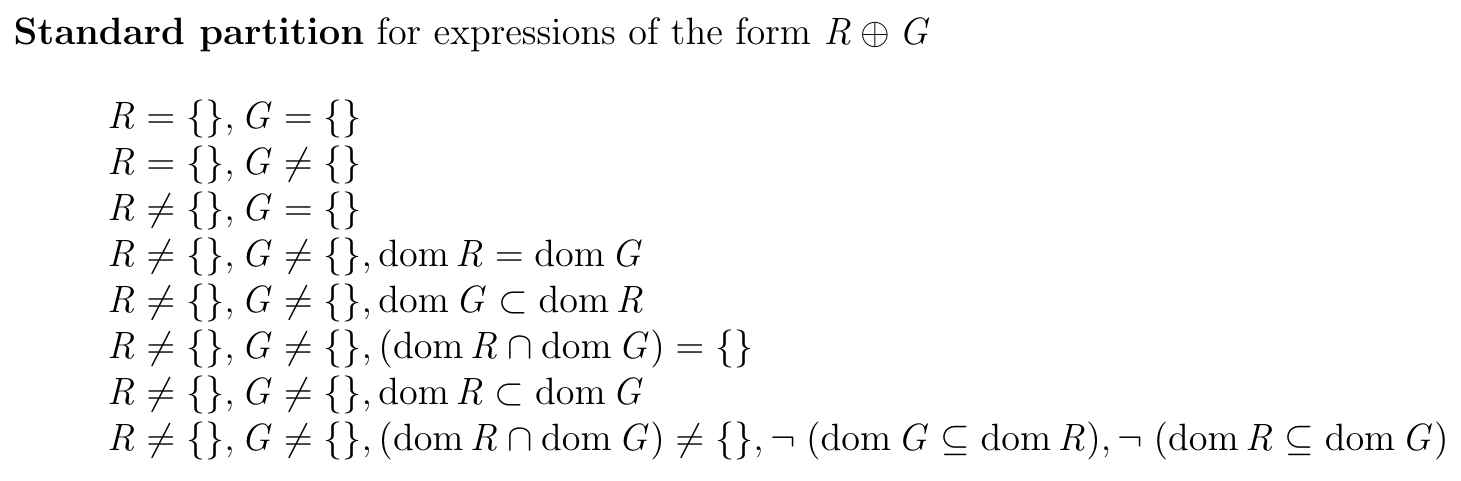
\includegraphics[width=0.8\linewidth]{sp_oplus.png}
\end{center}

donde $R = inscripciones$ y $G = \{alumno? \mapsto ((inscripciones~alumno?).1, estado?)\}$. A partir de esto se puede llegar a las siguiente conclusiones:
\begin{itemize}
    \item Por la definición de $G$ este conjunto tendrá siempre un elemento, siendo este la tupla \\ $(alumno?, ((inscripciones~alumno?).1, estado?))$, por lo que nunca se podrá dar que $G = \{\}$ y esto descarta los casos \emph{CerrarInscripcion\_FT\_12}, \emph{CerrarInscripcion\_FT\_14}, \emph{CerrarInscripcion\_FT\_20} y \emph{CerrarInscripcion\_FT\_22}.
    \item Otra consecuencia de que $G$ nunca podrá ser vacío es que dentro de su definición se consulta el valor asignado a $alumno?$ en la función $inscripciones$ lo que significa que $R \neq \{\}$, esto descarta los casos  \emph{CerrarInscripcion\_FT\_13} y \emph{CerrarInscripcion\_FT\_21}. Además otra consecuencia es que $alumno? \in \dom inscripciones$, esto implica $\dom G \subset \dom R \implies alumno? \in (\dom R \cap \dom G)$ y descarta los casos \emph{CerrarInscripcion\_FT\_17} y \emph{CerrarInscripcion\_FT\_25}.
    \item Otro caso de la partición estándar se da con la condición $R \neq \{\}, G \neq \{\}, \dom R \subset \dom G$. Para que esto suceda debería existir $alumno \in ALUMNO$ tal que $alumno \in \dom G \land alumno \notin \dom R$, pero si $alumno \in \dom G$ entonces por lo visto en el ítem anterior se tiene que dar $alumno \in \dom R$ y finalmente $\dom R \subset \dom G$ es una contradicción. Esto descarta los casos \emph{CerrarInscripcion\_SP\_18} y \emph{CerrarInscripcion\_SP\_26}.
    \item El último caso de la partición estándar viene dado por la condición $R \neq \{\}, G \neq \{\}, (\dom R \cap \dom G) \neq \{\}, \neg (\dom G \subseteq \dom R), \neg (\dom R \subseteq \dom G)$ y por los ítems anteriores sabemos que $\dom G \subset \dom R$ contradiciendo la condición. Esto descarta los casos \emph{CerrarInscripcion\_SP\_19} y \emph{CerrarInscripcion\_SP\_27}.
\end{itemize}

\subsubsection*{Esquemas de casos de pruebas generados}

Por último, los casos de prueba generados fueron los siguientes:

\begin{schema}{CerrarInscripcion\_ SP\_ 15\_ TCASE}\\
 CerrarInscripcion\_ SP\_ 15 
\where
 registrados = \{ aLUMNO1 \} \\
 inscripciones = \{ ( aLUMNO1 \mapsto ( 1 \mapsto repite ) ) \} \\
 estado? = promueve \\
 alumno? = aLUMNO1
\end{schema}

\begin{schema}{CerrarInscripcion\_ SP\_ 16\_ TCASE}\\
 CerrarInscripcion\_ SP\_ 16 
\where
 registrados = \{ aLUMNO1 \} \\
 inscripciones = \{ ( aLUMNO1 \mapsto ( 1 \mapsto repite ) ) , ( aLUMNO3 \mapsto ( 2 \mapsto promueve ) ) \} \\
 estado? = promueve \\
 alumno? = aLUMNO1
\end{schema}

\begin{schema}{CerrarInscripcion\_ SP\_ 23\_ TCASE}\\
 CerrarInscripcion\_ SP\_ 23 
\where
 registrados = \{ aLUMNO1 \} \\
 inscripciones = \{ ( aLUMNO1 \mapsto ( 1 \mapsto repite ) ) \} \\
 estado? = repite \\
 alumno? = aLUMNO1
\end{schema}

\begin{schema}{CerrarInscripcion\_ SP\_ 24\_ TCASE}\\
 CerrarInscripcion\_ SP\_ 24 
\where
 registrados = \{ aLUMNO1 \} \\
 inscripciones = \{ ( aLUMNO1 \mapsto ( 1 \mapsto repite ) ) , ( aLUMNO3 \mapsto ( 2 \mapsto promueve ) ) \} \\
 estado? = repite \\
 alumno? = aLUMNO1
\end{schema}

\begin{schema}{CerrarInscripcion\_ FT\_ 28\_ TCASE}\\
 CerrarInscripcion\_ FT\_ 28 
\where
 registrados =~\emptyset \\
 inscripciones =~\emptyset \\
 estado? = inscripto \\
 alumno? = aLUMNO1
\end{schema}

\begin{schema}{CerrarInscripcion\_ SP\_ 31\_ TCASE}\\
 CerrarInscripcion\_ SP\_ 31 
\where
 registrados =~\emptyset \\
 inscripciones =~\emptyset \\
 estado? = inscripto \\
 alumno? = aLUMNO1
\end{schema}

\begin{schema}{CerrarInscripcion\_ SP\_ 32\_ TCASE}\\
 CerrarInscripcion\_ SP\_ 32 
\where
 registrados = \{ aLUMNO1 \} \\
 inscripciones =~\emptyset \\
 estado? = inscripto \\
 alumno? = aLUMNO1
\end{schema}

\end{document}
